
\setcounter{section}{0}
\setcounter{figure}{0}
\graphicspath{{./figs/}{./figs/item-toyota/}}

\NewsTitle{Software Challenges for Automotive Cyber-Physical Systems}
\NewsAuthor{Huafeng Yu\\Toyota InfoTechnology Center, U.S.A.}

Cyber-Physical Systems (CPS) are well adopted in the automotive domain. Due to the mobility nature of vehicles, CPS are also required to be miniaturized in size, but required to provide powerful computing with low power consumption, particularly for connected and autonomous vehicles. In this trend, automotive CPS become increasingly complex, heterogeneous, and decentralized. Meanwhile, they are required to be more safe, reliable, optimized, and adaptive \cite{darpa-avm}, particularly for the control software in CPS \cite{broy06}. Since most of these systems are considered to be safety-critical, they require higher safety assurance along with the whole development process, from requirement, modeling, implementation, integration, to verification \& validation. 


However, the development of CPS, including electronics and their control software is generally achieved in an isolated and parallel manner by suppliers, according to the requirements provided by car manufacturers (OEMs) \cite{broy06}. Suppliers have the responsibility to assure the correctness, safety, and reliability of the components, whereas OEMs are in charge of requirements, final integration, evaluation and testing. This always leads to a gap between OEMs and suppliers. 

Design tools, methods, technologies, and processes are well matured in the automotive domain, but new challenges still emerge for the design of next generation connected and autonomous vehicles. In this paper, we briefly discuss current big challenges in the design of safety-critical software for automotive CPS, and then present a formal integration framework to partially address these challenges.


%in the design and integration of automotive CPS, particularly safety-critical software, still exist and XXX the fast and trustworthy development of automotive CPS and system-level integration.




%It is well known that the cost of  validation and resulting redesign increases exponentially if performed at the  late-phase implementation and integration. Therefore, system design is expected to be validated as early as possible, and design validation in an early phase has become one of the key approaches to reduce time to market constraints and the overall verification \& validation cost \cite{darpa-avm}. 

%High-level modeling languages, like SysML to capture the overall system specification,  and MATLAB/Simulink for the specification of control algorithms  are widely used to  model and validate at the early phases of design \cite{schmidt:2006-computer}. However, a plethora of high-level models and heterogeneous models of computation makes model integration a severe challenge for Model-Based Engineering (MBE).  
%This issue hampers the wider adoption  of model-based design approaches, particularly in the early-phase verification and validation at the system level. 
%
%To avoid aforementioned issues, a promising approach is the trustworthy \textit{virtual integration} \cite{giusto02, feiler09},  the validation of the virtually integrated model, and design refinement on the virtual prototype. However, at the level of virtual models, capturing  timing relations between component executions, real-time constraints, architectural constraints, and challenges of composability of actually implemented components, resource usage by the real components, etc., can be very challenging. Therefore, the virtual  model must have a representation of such implementation-specific constraints, and platform-specific yet essential properties represented in them. 
%
%Furthermore, since the component models are captured with heterogeneous models of computation, integration of such components at the virtual model level might not work at the implementation level unless platform-specific constraints are not captured in such models - beyond just their models of computation. For example, the platforms that these components would eventually run on, the properties of their communicating substrate (buses with different properties and timing) could highly influence their composability and correctness of composition. The real-time requirements, resource usage, etc., for the end-to-end system might also be influenced by the properties of the platform. Thus, virtual integration at just the functional model level is not a good approach to achieve high assurance design implementation. 


%Instead of providing isolated solutions to the aforementioned issues, we propose a model integration framework for the automotive domain, considering correct by construction, software architecture, view-based modeling and integration approach, and system optimization based on characteristics related to specific platforms.
%We adopt formal specification in an early stage of design at the modeling level. The formal specification is based on multi-clock timing \cite{Guernic:2002} and formal contract \cite{meyer:1992-computer}, extracted from informal automotive requirements, to enable a correct composition of system models. 
%%%% timing
%Multi-clock timing specification are based on the modeling of synchrony and time as software and hardware events, and are related to synchronization in an architecture specification. 
%Compared to real time, synchronous logical time, applied on both software and architecture,  provides an algebraic framework in which both event-driven and time-triggered execution policies can be specified.
%%%% contract
%The formal contracts, used for describing the functional and non-functional specifications of the components, take into account the architecture and platform models as well as their related properties. A dual design methodology, called \textit{Inside-out} and \textit{Outside-in}, is proposed to formally address the decomposition and composition of contracts such that both systems (from car manufacturers) and subsystems (from suppliers) satisfy all contracts.


%In the framework, software architecture is explicitly specified with a standardized architecture description language, AADL~\cite{AADLv2-AS5506A}. From a view-based design approach, behavioral, architectural, and timing views of the system \cite{Guernic:2002} are all considered, along with the compositional view of system models. Multiple formalism and languages are adopted for each view, for example, Simulink for behavioral view, AADL for architectural view, contract for compositional view and synchronous languages for timing view. Formal evaluation of the system is first performed on each view in a separated way, and then in an integrated way in our proposed integration framework. 





%\input{doc/challenges}
\section{Design Challenges}


%In this section, the challenges of automotive model-based system integration will be briefly presented first.
\vspace{0.6em}
\indent\indent\textbf{Formal specification.}
Automotive specification is mainly based on informal requirements. As a consequence, it frequently leads to ambiguity and misunderstanding between OEMs and their suppliers. However, a complete formal specification is also impossible due to the limitations in language expression, time, cost, performance, etc. Therefore, an appropriate formal specification, created in an incremental, composable, and reusable manner is indispensable for the building of reliable model-based integration and formal verification. This specification is expected to be independent from languages, tools, and platforms for wider adaptation and good reusability in industry.

\vspace{0.6em}
%%%%%%%%%%%%%%%%%%%%%%%
\textbf{Modeling.}
In system design, various general or domain-specific modeling languages are used \cite{muller-glaser:2004-tcst} because of different needs, including different application domains, performance, expertise, cost, etc.. For instance, UML is used as a general modeling language, and SysML is adopted in systems engineering related applications. MATLAB/Simulink and Modelica are used as domain-specific modeling languages in a wide span of domains, while SCADE is mostly used for safety-critical systems and requires a strong background in rigorous design. Each language and its associated tool-set provide good support for their own development process from modeling to implementation. However a virtual integration using multiple languages and models turns out to be complicated, ambiguous and unpredictable. 

\vspace{0.6em}
\textbf{Architecture modeling.}
Software architecture \cite{shaw1996software} was not considered essential, thus rarely formalized in conventional automotive design processes. Consequently, it generally leads to a manual, error-prone, time-consuming architecture exploration and validation. 
To avoid this problem, formalization, formal reasoning, and early-phase exploration are required, along with explicit quality attributes associated with particular architectural entities. 
Currently, architectural aspects of the system are not well expressed by general modeling languages. Architecture description languages, such as AADL\cite{AADLv2-AS5506A}, 
AUTOSAR~\cite{AUTOSAR} and EAST-ADL~\cite{EAST-ADL} were therefore proposed for embedded systems, especially avionic and automotive systems.  
A system-level design, considering both architecture and behavior, is becoming a promising solution to promote the virtual integration solution for embedded control systems \cite{feiler09, yu:2013-jsa}.



\vspace{0.6em}
\textbf{Timing specification.}
Semantics interoperability is one of the main issues in the composition of models, due to semantic dissimilarity between models and their inherent formalism, particularly for timing specification. The timing issue is among the most significant concerns in automotive system design \cite{broy06, yu:2013-jsa}. In general, the timing issue becomes more explicit when architecture is considered and the system is integrated, due to the gap between software and architecture design. To cope with timing-related semantics interoperability, one of the feasible solutions is to have a common formal model as the intermediate semantic model, and translate all other models into this common model. The intermediate model provides the formal semantics, based on which, the  expected properties of the original models and their integration are checked. An example can be found in \cite{YU:2011:INRIA-00536907:1}. However, this approach requires a semantics preservation in the model translation, which is not practical in most cases. Another solution is related to unified formalism 
\cite{mathaikutty:2005-fdl, lee:2006-cadics}. 
However, this approach is more theoretical and not yet well applied in industry.

\vspace{0.6em}
\textbf{Integration frameworks.}
System integration is a big challenge due to isolated development, lack of integration and architecture specification, late phase for the integration, etc. A new trend to reduce integration issue is model-based integration. Research on model-based system integration has been discussed with regard to cyber-physical systems \cite{sztipanovits:2012-pieee}; Service-oriented Architecture \cite{rossignol:2013-chap}; and heterogeneous models integration and simulation \cite{eker:2003-pieee}. In addition, AUTOSAR\cite{AUTOSAR} aims at component and platform-level integration for automotive systems, and System Architecture Virtual Integration (SAVI) program \cite{feiler09} targets avionic system integration. 
However due to multiple challenges in the model integration, integration frameworks, as opposed to specific integration solution, are becoming increasingly important. These frameworks are expected to consider formal specification and analysis, multi-view, and orthogonal attributes of the system, as well as \textit{correct by construction} and \textit{separation of concerns}, to reduce design complexity and validation time. 


\vspace{0.6em}
\textbf{Certification.}
In addition to testing or verification methods, automotive engineers also need to consider certification. The developed vehicles are required to be certified to be safe by using the artifacts and evidences produced throughout the development cycle. Such a certification process helps to increase the safety confidence of the developed software and reduce OEM's liability. However, software certification in automotive domain is not yet well established, e.g., safety-relevant standards are not yet well defined, and the automotive safety standard ISO26262 is mainly based on process, lacking of support to product-oriented certification; lack of guidance and supervision from regulators or government agencies, unlike other domains of aviation and medical devices.

\vspace{0.6em}
\textbf{Security.}
Recent reports on security-related vehicle hacking involve various systems in many models from different OEM's \cite{Schneider15} \cite{Harris2015}. A series of successful hacking activities of current car models show the lack of system-level security consideration in  vehicle hardware and software design, integration, certification, and production. These concerns also raise to US political level \cite{Markey15}. Integration of security mechanisms in vehicles involves not only computing resources but also other features, like safety, reliability, etc., which finally make it a big challenge.

\vspace{0.6em}
\textbf{Tool support.}
Tool support of MBE is one of the key concerns from an industry adoption viewpoint \cite{broy:2010-pieee}.  Specific model-based tool chains were developed as solutions, such as \cite{Armengaud11b}, for safety-relevant automotive embedded systems. However, the lack of serious consideration of formal aspects and integration semantics in these tool chains limits their support for a reliable integration. Tool qualification is another concern related to certification.



In the following, we summarize our current contribution, aiming at addressing previous issues in the context of model-based integration for automotive software control systems. This work is mainly inspired from \cite{yu:2013-jsa, ma13, feiler09, darpa-avm, sztipanovits:2012-pieee, broy:2010-pieee}.



%\input{doc/framework}
\section{The VIF Integration Framework}

%The proposed framework follows the concept of a previous research project, dedicated to the system-level co-modeling, analysis, verification and simulation in the avionic domain \cite{YU:2011:INRIA-00536907:1, yu:2013-jsa}, where AADL and MATLAB/Simulink have been used to model a simplified Airbus A350 doors management system. A formal model of computation (MoC), called Polychrony \cite{Guernic:2002}, was adopted as a supporting semantic model to enable an unambiguous and trustworthy integration. The later formal analysis, verification, and scheduling were mainly performed on the basis of the same MoC. 

Based on the previous exploration \cite{YU:2011:INRIA-00536907:1, yu:2013-jsa}, our current research mainly copes with a formal virtual integration framework for next-generation design of automotive control software. Our framework, called VIF (Virtual Integration Framework), promotes \textit{correct by construction} in the early design phase, rather than a posteriori \textit{Verification \& Validation}.
The main research topics involved in this framework include: formal timing specification, architecture modeling, design by contract, semantics interoperability and system optimization, as well as specification and modeling for different views and properties of the system, such as behavior, architecture, composition, and timing. All these techniques are adopted in the framework as key solutions to the challenges presented.


Formal timing specification and design by contract play a core role in the trustworthy model integration in our approach. 
%%%% timing
High-level, formalized, multi-clock timing specification, considered as a central topic, is to be defined, observed and analyzed, based on software architecture. 
%Considering abstraction in the system design, we advocate the modeling of synchrony and time as software and hardware events, which are related to synchronization in an architecture. 
%Compared to real time, synchronous logical time, applied on both software and architecture,  provides an algebraic framework in which both event-driven and time-triggered execution policies can be specified.
%%%%
The formal contracts, used for describing the functional and non-func\-tional specifications of the components, consider the  architecture and platform models as well as their associated properties. A dual design methodology, called \textit{Inside-out} and \textit{Outside-in}, is proposed, where the first part addresses decomposition of a contract into sub-contracts, such that the latter can independently be given to automotive suppliers, instead of natural language specifications. The second part deals with a reliable integration of sub-systems to obtain the required system satisfying all contracts.
%Timing specification and formal contract will be detailed in Section~\ref{sec:architecture} and Section~\ref{sec:contract} respectively.

\begin{figure}[htbp]
	\centering
    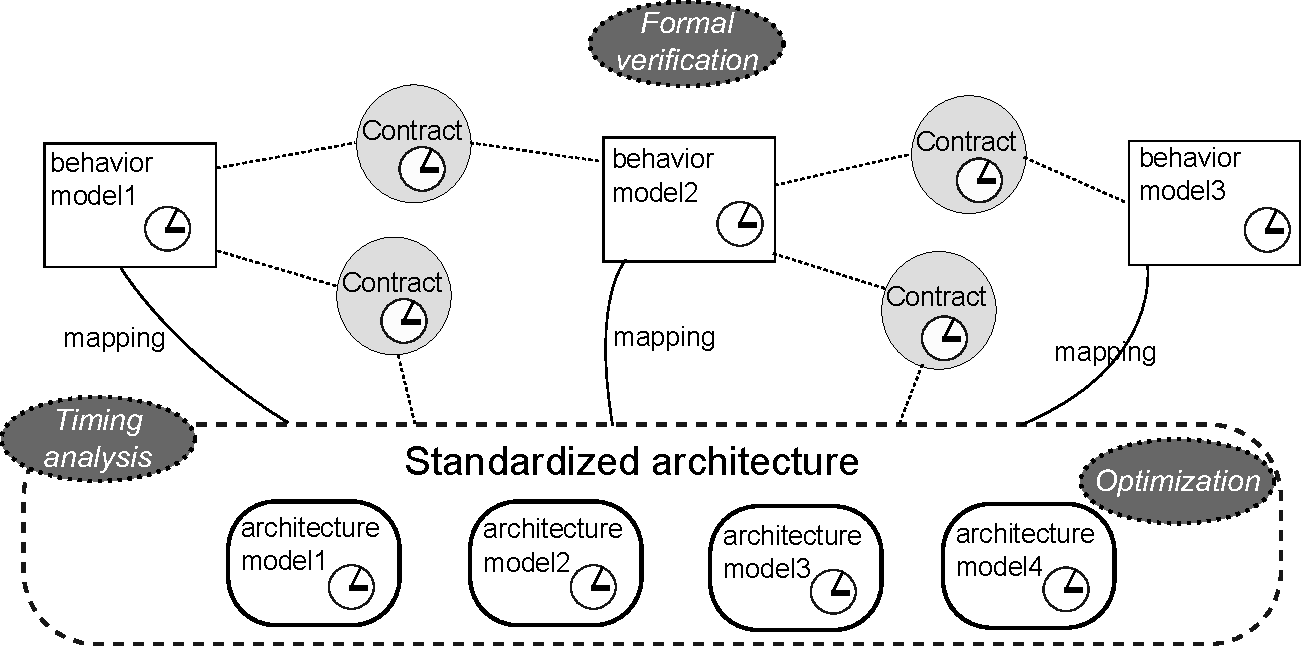
\includegraphics[width=0.6\linewidth]{framework}
	\caption{An overview of the integration framework}
	\label{fig:framework}
\end{figure}

Figure~\ref{fig:framework} briefly illustrates the integration framework. High-level automotive requirements are initially analyzed, from which \textit{formalizable} requirements are extracted, according to the technical formalizability and verifiability. 
These requirements are then used to create formal contracts for properties of timing, safety, performance, etc. In addition to these aspects, multiple modeling languages are applied for different views of the system in the framework, for instance, AADL for architecture modeling and Simulink for behavior modeling. 
Both timing specification and contracts are defined on these models, to enable a reliable integration. 
In the final step, behavior models are mapped onto the architecture model, considering pre-defined optimization criteria.

\section{Conclusion}
We briefly presented current big challenges in the design of software in automotive cyber-physical systems, including: formal specification, modeling, architecture, timing specification, integration framework, certification, security, and tool support. However, isolated software development, without consideration of system-level requirements and integration, is not enough. More rigorous system-level design methodologies are required to enable and enhance the system-level requirements on safety, reliability, performance, and security, etc. As a potential solution to partially address previous challenges, we  exhibited our proposed formal integration work, VIF, with focus on architecture modeling, timing specification, and integration correctness.

\bibliographystyle{plain}
\begin{thebibliography}{10}

\bibitem{Armengaud11b}
E.~Armengaud, M.~Zoier, et~al.
\newblock {``Model-based Toolchain for the Efficient Development of Safety-Relevant Automotive Embedded Systems''}.
\newblock In {\em SAE World Congress \& Exhibition}, 2011.

\bibitem{AUTOSAR}
{AUTOSAR (AUTomotive Open System ARchitecture)}.
\newblock \url{http://www.autosar.org/}.

\bibitem{broy06}
M.~Broy.
\newblock {``Challenges in Automotive Software Engineering''}.
\newblock In {\em International Conference on Software Engineering (ICSE)},
  2006.

\bibitem{broy:2010-pieee}
M.~Broy, M.~Feilkas, M.~Herrmannsdoerfer, S.~Merenda, and D.~Ratiu.
\newblock {``Seamless Model-Based Development: From Isolated Tools to Integrated Model Engineering Environments''}.
\newblock {\em Proceedings of the IEEE}, 98(4):526--545, 2010.

\bibitem{darpa-avm}
DARPA.
\newblock {``Adaptive Vehicle Make (AVM) Program''}.
\newblock \url{http://www.darpa.mil/Our\_Work/TTO/Programs}.

\bibitem{EAST-ADL}
{EAST-ADL}.
\newblock \url{http://www.east-adl.info}.

\bibitem{eker:2003-pieee}
J.~Eker, J.W. Janneck, E.A. Lee, J.~Liu, X.~Liu, J.~Ludvig, S.~Neuendorffer,
  S.~Sachs, and Y.~Xiong.
\newblock {``Taming Heterogeneity - the Ptolemy Approach''}.
\newblock {\em Proceedings of the IEEE}, 91(1):127--144, 2003.

\bibitem{feiler09}
P.-H. Feiler, J.~Hansson, D.~{de Niz}, and L.~Wrage.
\newblock {``System Architecture Virtual Integration: An Industrial Case Study''}.
\newblock Technical report, Software Engineering Institute, 2009.
\newblock CMU/SEI-2009-TR-017.

\bibitem{Harris2015}
M.~Harris.
\newblock ``Researcher hacks self-driving car sensors''.
\newblock {\em IEEE Spectrum}, 2015.

\bibitem{lee:2006-cadics}
E.~A. Lee and A.~Sangiovanni-Vincentelli.
\newblock {``A Framework for Comparing Models of Computation''}.
\newblock {\em IEEE Transactions on Computer-Aided Design of Integrated
  Circuits and Systems}, 17(12):1217--1229, 2006.

\bibitem{ma13}
Y.~Ma, H.~Yu, T.~Gautier, P.~{Le Guernic}, J.-P. Talpin, L.~Besnard, and
  M.~Heitz.
\newblock {``Toward Polychronous Analysis and Validation for Timed Software Architectures in AADL''}.
\newblock In {\em Design, Automation, and Test in Europe (DATE)}, pages
  1173--1178, 2013.

\bibitem{Markey15}
E.~Markey.
\newblock Tracking \& hacking: Security \& privacy gaps put american drivers at
  risk, 2015.

\bibitem{mathaikutty:2005-fdl}
D.~Mathaikutty, H.~Patel, S.~Shukla, and A.~Jantsch.
\newblock {``Modelling Environment for Heterogeneous Systems based on MoCs''}.
\newblock In {\em Forum on specification and Design Languages (FDL)}, pages
  291--303, 2005.

\bibitem{muller-glaser:2004-tcst}
K.D. M\"uller-Glaser, G.~Frick, E.~Sax, and M.~K\"uhl.
\newblock {``Multiparadigm Modeling in Embedded Systems Design''}.
\newblock {\em IEEE Transactions on Control Systems Technology},
  12(2):279--292, 2004.

\bibitem{rossignol:2013-chap}
A.~Rossignol.
\newblock {``The Reference Technology Platform''}.
\newblock In {\em CESAR - Cost-efficient Methods and Processes for
  Safety-relevant Embedded Systems}. Springer, 2013.

\bibitem{AADLv2-AS5506A}
{SAE Aerospace (Society of Automotive Engineers)}.
\newblock {``Aerospace Standard AS5506A: Architecture Analysis and Design Language (AADL)''}.
\newblock {\em SAE AS5506A}, 2009.

\bibitem{Schneider15}
D.~Schneider.
\newblock Jeep hacking 101.
\newblock {\em IEEE Spectrum}, 2015.

\bibitem{shaw1996software}
M.~Shaw and D.~Garlan.
\newblock {``Software Architecture: Perspectives on an Emerging Discipline''}.
\newblock {\em Prentice Hall Englewood Cliffs}, 1996.

\bibitem{sztipanovits:2012-pieee}
J.~Sztipanovits, X.~D. Koutsoukos, G.~Karsai, N.~Kottenstette, P.J. Antsaklis,
  V.~Gupta, B.~Goodwine, J.S. Baras, and S.~Wang.
\newblock {``Toward a Science of Cyber-Physical System Integration''}.
\newblock {\em Proceedings of the IEEE}, 100(1):29--44, 2012.

\bibitem{yu:2013-jsa}
H.~Yu, Y.~Ma, T.~Gautier, L.~Besnard, J.-P. Talpin, and P.~{Le Guernic}.
\newblock {``Polychronous Modeling, Analysis, Verification and Simulation for Timed Software Architectures''}.
\newblock {\em Journal of Systems Architecture (JSA)}, 59(10):1157--1170, 2013.

\bibitem{YU:2011:INRIA-00536907:1}
{H.} {Y}u, {Y.} {M}a, {Y.} {G}louche, {J.}-{P.} {T}alpin, {L.} {B}esnard, {T.}
  {G}autier, {P.} {L}e {G}uernic, {A.} {T}oom, and {O.} {L}aurent.
\newblock ``{S}ystem-level {C}o-simulation of {I}ntegrated {A}vionics {U}sing {P}olychrony''.
\newblock In {\em ACM Symposium on Applied Computing (SAC)}, 2011.

\end{thebibliography}
